\documentclass{article}
\usepackage{amsmath}
\usepackage{amsfonts}
\usepackage{algorithm2e}
\usepackage{color}
\usepackage{graphicx}
\usepackage[export]{adjustbox}


\title{Generalized Reed-Solomon Codes}
\author{John McCall\\Course: Math 4901\\Adviser: Peter Dolan\\Second Reader: David Roberts}

\begin{document}
\RestyleAlgo{boxruled}
\definecolor{greyCode}{gray}{.75}

\newcommand{\f}[1]{
	\colorbox{greyCode}{\texttt{#1}}
}

\maketitle

\section{Abstract}
Error correcting codes are used to correct any errors which may occur in a data transmission. Generalized Reed-Solomon (GRS) codes are a class of error correcting code. They are utilized in real world applications such as CD-roms and deep space communications, due to their ability to recover even when a large chunk of data has been compromised. While no error correcting code is perfect, the ability to correct any number of errors during data transmission is incredibly useful. This paper describes generalized Reed-Solomon codes and goes into detail about the process of encoding and decoding a GRS code.

\section{Introduction}
Communication plays a huge role in today's society. Electronic forms of communication become more prevalent every year. Whether it is listening to a CD in the car, reading an article on the internet, or talking with a friend via a cell phone, electronic communication impacts our everyday lives. However, these forms of communication are not always perfect. For instance, that CD could become scratched, corrupting some of its data. Error correcting codes are a way of coping with corruption. 

The idea behind error correcting codes is to encode and transmit the data with a sufficient amount of redundancy to be able to reconstruct data that may become lost or corrupted. This is why that even when a CD gets some minor scratches it will still be able to play perfectly. These codes are not perfect. If a scratch is too large, some of the data will be irrecoverable and there will be a noticeable effect on the music playing.

Reed-Solomon codes are error correcting codes. They were first introduced in 1960 by I.S. Reed and G. Solomon~\cite{RS:1960}. These codes are somewhat rare in that they have both useful practical applications and an interesting mathematical foundation. Today, Reed-Solomon codes are used in many applications such as CD players and deep-space communications.

In Section 3 we will provide the necessary abstract algebra background to understand the remainder of the paper. Section 4 will introduce coding theory and give examples of some codes. In Section 5 we will go into detail about Generalized Reed-Solomon codes and will walk through an example.

\section{Background}
This section will provide all the necessary background in abstract algebra that is needed to understand Generalized Reed-Solomon codes. Specifically it will define groups, cyclic groups, rings and fields. %Introduce the finite field $\mathbb{F}_{2}$ as well as the extension field $\mathbb{F}_{2^{m}}$. Then it will describe how addition and multiplication behave in this field.

\subsection{Groups, Rings, and Fields}
A \textit{group} is a set, $G$, paired with a binary operation, usually denoted as $+ \text{ or } \cdot$, and referred to as addition and multiplication. For now we will use the multiplicative notation. A group must have the following properties.
\begin{enumerate}
  \item $G$ must be closed under the operation. In otherwords, for any $a, b \in G, a \cdot b \in G$ as well.
  \item The operation must be associative. So for all $a,b,c \in G$ we have $(a \cdot b) \cdot c = a \cdot (b \cdot c)$.
  \item There must be an identity element. This means that there exists an element $e \in G$ such that for all $a \in G, a \cdot e = e \cdot a \ a$. Traditionally, $e$ is written as $0$ if we are using $+$ to denote our operation or as $1$ if we are using $\cdot$.
  \item Inverse elements must exist. So for all $a \in G$ there exists an element $a^{-1} \in G$ such that $a \cdot a^{-1} = a^{-1} \cdot a = e$, the identity element.
\end{enumerate}
It is important to note that the operation does not need to be commutative. If it is commutative that is called an \textit{abelian group}. An example of a group would be $\mathbb{Q}$ under addition. It is easy to see that the rational numbers under normal addition satisfies all of the above properties and is a group. Another example would be $\mathbb{Q}^{*}$, the rationals with zero removed, under multiplication. Zero needed to be removed in this case because it has no multiplicative inverse.

An element $a \in G$ is called a \textit{generator} or a \textit{primitive element} of $G$ if $\{a^{n} | n \in \mathbb{Z}\} = G$. In other words if we take $a$ and multiply it by itself repeatedly, the set of products will be equal to the set $G$. Any group which has a generator is called a \textit{cyclic group}.

A \textit{ring} is a set $R$, paired with two binary operations, usually denoted $+ \text{ and } \cdot$ and referred to as addition and multiplication, such that the following properties hold.
\begin{enumerate}
  \item $R$ under addition is an abelian group.
  \item Multiplication is associative.
  \item The two distributive laws always hold true. In other words, $a \cdot (b + c) = (a \cdot b) + (a \cdot c)$ and $(b + c) \cdot a = (b \cdot a) + (c \cdot a)$.
\end{enumerate}
The multiplication does not have to be commutative. If it is, then the ring is called a \textit{commutative ring}. Another thing to notice is that multiplicative inverses are not required in a ring. An element that does have a multiplicative inverse is called a \textit{unit}. If a ring is commutative and every non-zero element is a unit, that is, every element has a multiplicative inverse then that ring is called a \textit{field}. The integers, along with normal addition and multiplication, are an example of a commutative ring. However, they are not a field since not every element has a multiplicative inverse. The solution to this is to add fractions, giving every element a multiplicative inverse. Thus, the rational numbers are a field. 

We use the notation $\mathbb{F}[x]$ to denote all polynomials with coefficients in the field $\mathbb{F}$. Polynomials with rational coefficients would be denoted $\mathbb{Q}[x]$, polynomials with real coefficients would be denoted $\mathbb{R}[x]$. We write $\mathbb{F}[x]_{k}$ to denote all polynomials with coefficients in $\mathbb{F}$ with degree less than $k$.

\subsection{Defining $\mathbb{F}_{64}$}
The field which we will focus on in this paper is $\mathbb{F}_{64}$. The finite field of 64 elements.
For our purposes, the elements of this field will be 64 ASCII characters, shown in Appendix A. The elements include all capital letters, the numbers zero through nine, as well as some punctuation. These characters where chosen specifically to make encoding easier. Since these symbols can be hard to distinguish from actual text, the symbols will be given a grey background. For example: $\f{A}, \f{1}, \f{\#}$ are all elements in $\mathbb{F}_{64}$.

These elements can be represented as binary strings, which in turn represent polynomials in $\mathbb{F}_2[x]_{6}$. In other words, polynomials with coefficients that are either zero or one that are of degree five or less. For example, $\f{\#}$ can be written as the binary string \texttt{11}. This binary string represents the polynomial $x + 1$. The symbol $\f{\$}$ corresponds to the binary string \texttt{100}, which gives us the polynomial $x^2$.

\subsubsection{Addition in $\mathbb{F}_{64}$}
To perform addition in $\mathbb{F}_{64}$, we first convert the elements being added to their polynomial form. Then we simply add those polynomials, keeping in mind that the coefficients are in $\mathbb{F}_2$. To illustrate this, take $\f{!} + \f{\#}$. This becomes: $1 + (x + 1)$. Doing the addition in $\mathbb{F}_2$ yields $x$, which represents the element $\f{"}$. So, $\f{!} + \f{\#} = \f{"}$. A complete addition table for $\mathbb{F}_{64}$ can be found in Appendix~B.

\subsubsection{Multiplication in $\mathbb{F}_{64}$}
Similarly to addition, we use the polynomial representation of our elements to multiply them. Let us multiply $\f{\#}$ by itself. 
\begin{center}
$\f{\#} * \f{\#} = (x + 1) * (x + 1) = x^2 + x + x + 1 = x^2 + 1 = \f{\%}$.
\end{center}

A problem that arises when doing multiplication is that it is possible to produce a polynomial that is higher than degree 5. For instance:
\begin{center}
$\f{\%} * \f{0} = (x^2 + 1) * (x^4) = x^6 + x^4$
\end{center}

When this occurs we use the the irreducible polynomial $x^6 + x + 1$ to reduce the power. In $\mathbb{F}_2$ we can rewrite that polynomial as $x^6 = x + 1$. We can then substitute this value into our product to lower the degree.
\begin{center}
$x^6 + x^4 = (x+1) + x^4 = x^4 + x + 1 = \f{3}$
\end{center}

A complete multiplication table can be found in Appendix B. In addition to this there is also a grey-scale multiplication table included in Appendix B. The grey-scale table helps to illustrate patterns that appear in the multiplication that are hard to see using the normal table. Most notably, it is easy to see multiplication is commutative using the grey-scale table because the table is symmetrical along the main diagonal.

\subsubsection{Polynomials over $\mathbb{F}_{64}$}
Let us define $\mathbb{F}_{64}[x]$ to be all polynomials with coefficients in $\mathbb{F}_{64}$. We can perform all of the usual polynomial operations using the addition and multiplication methods defined above including: addition, multiplication, substitution, and taking the derivative. For example, let
\begin{center}
$f(x) = \f{!}x^{3} + \f{!}x^{2} + \f{\#}x + \f{/}$
\end{center}

then
\begin{equation*}
\begin{split}
f(\f{A}) & = (\f{!} * \f{A}^{3}) + (\f{!} * \f{A}^{2}) + (\f{\#} * \f{A}) + \f{/} \\
& = (\f{!} * \f{Q}) + \f{!} + (\f{\#} * \f{Y}) + \f{/} \\
& = \f{Q} + \f{Y} + \f{@} + \f{/} \\
& = \f{G}
\end{split}
\end{equation*}

The derivative, $f'(x)$, would equal

\begin{equation*}
\begin{split}
f'(x) & = 3 * \f{!}x^{2} + 2 * \f{!}x + \f{\#} \\
& = (\f{!} + \f{!} + \f{!})x^{2} + (\f{!} + \f{!})x + \f{\#} \\
& = \f{!}x^{2} + \f{\#}
\end{split}
\end{equation*}


\section{Codes}
A \textit{code} is a rule for converting information (usually a letter or word) into another representation. \textit{Encoding} is the actual act of conversion. A simple code would be to map each letter of the alphabet to a number. For instance, ``A" maps to ``1", ``B" maps to ``2", etc. In this example, the letters are our \textit{source alphabet}, and the numbers are our \textit{target alphabet}. To encode the word ``ALGEBRA" we would simply replace all the letters with the appropriate numbers. In this case, ``1,12,7,5,2,17,1" is the result. The act of \textit{decoding} reverses the code and returns the word to its original state. 

Codes are very useful when storing data, or transmitting it over long distances, as they provide an easy, consistent, way of representing data. However, this data may be corrupted in transmission. \textit{Random errors} are a type of error that corrupts individual symbols during transmissions. Corruption, in this context, means changing the symbol to another symbol in our alphabet, or deleting a symbol all together. Going back to our example, if two random errors occur during transmission, our word may arrive as: ``1,17,7,1,2,17,1". A ``2" was replaced with a ``7" and a ``5" was replaced with a ``1". As a result our decoded word is: ``ARGABRA". A \textit{burst error} is when a chunk of symbols in a row become corrupted. These can be particularly troublesome as they can corrupt a large portion of the data, and are common in several types of communication channels.

Codes that can detect these error are called \textit{error detecting} codes. Codes that can correct these errors are called \textit{error correcting} codes. There is no perfect code which can correct or detect all errors. The ability to correct even a small amount of errors is better than the alternative of having to retransmit the data every time an error occurs.

Before examining Reed-Solomon codes, we will discuss a simpler code. Cyclic Redundancy Check is a good code to start with because it introduces several important ideas in coding theory. 

\subsection{Cyclic Redundancy Check}
An example of an actual code, used in computer hard drives, is a \textit{cyclic redundancy check (CRC)}. A CRC is a type of error detecting code used to detect accidental changes in data. To detect an error, a fixed length \textit{check value} is appended to the end of the message. The check value is based on the remainder of a polynomial division of the messages contents. When the message is received the check value is recomputed and the appropriate measures to fix the corruption can be taken if the two values do not match.

CRCs are commonly used because they are easy to implement in binary hardware, easy to analyze, and are quite good at detecting burst errors. Usually, an $n$-bit CRC used on an arbitrary length message will detect any single burst error less than or equal to $n$ bits and will detect a fraction $1 - 2^{-n}$ of all longer burst errors~\cite{wiki:crc}.

The specification of a CRC code requires a \textit{generator polynomial}, which is an irreducible polynomial of degree $n$. This polynomial is the divisor in polynomial long division, the dividend is the message, the quotient is thrown away, and the remainder becomes the result. It is important to note that the coefficients of the polynomial are computed using the carry-less arithmetic of a 
finite field. Most CRCs use the finite field $\mathbb{F}_{2}$ in practice as this field only has two elements, 0 and 1, which meshes nicely with the architecture of computers.

A CRC is called an $n$-bit CRC when its check value has $n$ bits. Any $n$ has multiple CRCs, each with a different polynomial. Any such polynomial has highest degree $n$, which means that it has $n + 1$ terms, and that its encoding requires $n + 1$ bits. A CRC and associated polynomial are given a name of the form CRC-$n$-XXX. The simplest CRC is CRC-1 and it uses the generator polynomial $x + 1$. This is also called a parity bit, which is the simplest form of error detection.

\subsubsection{Application and Integrity}
A device that implements a CRC calculates the check value for each data block to be sent or stored and appends it to the end of the block. When a block is read or received the device does one of two things. It either recalculates the check value of the data block and compares it to the check value received, or it performs a CRC on the entire block and checks that the result is zero. If the check values do not match, then errors have been successfully detected in the block. Due to the nature of error-checking, it is possible that some errors may remain undetected, even if the check values match. 

CRCs are designed to protect accidental errors incurred from communication channels, and can give assurance of the integrity of delivered messages. CRCs are not suitable when it comes to protecting against intentional modification of data for several reasons. One reason is that there is no authentication so an attacker can edit the message and recompute the CRC without being detected.

\subsubsection{Computing a CRC}
To compute an $n$-bit binary CRC, start with the message encoded in binary:
\begin{verbatim}
1100101
\end{verbatim}
This is padded with $n$ zeroes, corresponding to the bit length $n$ of the CRC. The first calculation for a 3-bit CRC is as follows:
\begin{verbatim}
1100101 000 <--- input padded with 3 bits
1011               <--- divisor (4 bits) 
------------------
0111101 000
\end{verbatim}
If the input bit above the leftmost divisor bit is 0, do nothing. If the bit is 1, the divisor is XORed with the input. The divisor is then shifted one bit to the right. This process is repeated until the divisor reaches the right most bit of the input. The calculation in its entirety is:
\begin{verbatim}
1100101 000 <--- input padded with 3 bits
1011        <--- divisor
0111101 000 <--- result
 1011       <--- divisor ...
0010001 000
  1011
0000111 000
    101 1
0000010 100
     10 11
-------------     
0000000 010 <--- remainder (3 bits)                    
\end{verbatim}

In this case the leftmost bit in the divisor zeroes out all the bits in the input so all that's left is the remainder. To check the validity of the received message simply perform the computation again, but instead of padding the input with zeroes, add the check value instead. If there are no errors the remainder after this computation should be zero. If the remainder is not zero that means that there were errors in the received message.
\begin{verbatim}
1100101 010  <-- No errors          Errors -->  1010101 010
1011	                                            1011
0111101 010                                      0001101 010
 1011                                               1011 
0010001 010                                      0000110 010
  1011                                               101 1
0000111 010                                      0000011 110
    101 1                                             10 11
0000010 110                                      0000001 000
     10 11                                             1 011
-------------                                   -------------
0000000 000	          <-- Remainder -->          0000000 011
\end{verbatim}

\subsection{Linear Codes}
A \textit{linear code} of length $n$ and rank $k$ is a linear subspace $C$ with dimension $k$ of the vector space $\mathbb{F}^{n}_{q}$ where $\mathbb{F}_{q}$ is the finite field with $q$ elements. For our purposes $q = 2^m$. The vectors in $C$ are called \textit{codewords}. The \textit{weight} of a codeword is the number of its nonzero elements. The \textit{distance} between two codewords is the number of elements in which they differ. This is called the \textit{Hamming distance}.

Since $C$ is a linear subspace of $\mathbb{F}^{n}_{q}$, $C$ can be represented by a basis. A matrix can be constructed from this basis where each row in the matrix is an element from the basis set. This matrix is called the \textit{generator matrix} of $C$.

The \textit{dual code} of a code $C$, denoted $C^{\perp}$ is the code
\begin{center}
$C^{\perp} = \{\textbf{x} \in F^{n} \mid \textbf{x} \cdot \textbf{c} = 0, \text{ for all } c \in C\}$
\end{center}
where $\textbf{x} \cdot \textbf{c}$ is the usual dot product, generalized to $\mathbb{F}_{q}^{n}$. If $C$ is a linear code, then $C^{\perp \perp} = C$. Dual codes are useful because they possess the property that if $G$ is a generator matrix for $C$ then $\textbf{x}$ is in $C$ if and only if $G\textbf{x}^{\mathsf{T}} = \textbf{0}$.

The generator matrix $H$ for the dual code $C^{\perp}$ of linear code $C$ is called a \textit{check matrix} for $C$. For us, $C^{\perp \perp} = C$, so we can use the check matrix $H$ for $C$ to define $C$ as:
\begin{center}
$C = \{\textbf{x} \mid H\textbf{x}^{\mathsf{T}} = \textbf{0}\}$.
\end{center}
Often a code is defined using a check matrix. %[Insert example here?]

\section{Reed-Solomon Codes}
Reed-Solomon codes are a linear code. An $n$ length and $k$ dimension Reed-Solomon code is capable of correcting $\left \lfloor{\dfrac{n - k}{2}}\right \rfloor$ symbol errors. Because of this RS codes are quite adept at correcting burst errors. For instance, lets say we have a Reed-Solomon code of length $n = 128$ and dimension $k = 120$. Each symbol of our code will be made up of eight bits. Since $n - k = 128 - 120 = 8$ this means that we can correct any four symbol errors in our block of 128 symbols. This is true even if they are four consecutive symbols, as could happen due to a burst error.

A message encoded using a Reed-Solomon code is a polynomial with the message embedded in the coefficients. This is called the \textit{message polynomial}, $m(x)$. In general, $m(x) \in F[x]_{k}$ where $F$ is a field. However, we will be working in $\mathbb{F}_{64}$ for the remainder of the paper so we will have $m(x) \in \mathbb{F}_{64}[x]_{k}$. Say the message we want to encode is: ``THIS IS MAJOR TOM". Then our message polynomial is:
\begin{center}
$m(x) = \f{T} + \f{H}x + \f{I}x^{2} + \f{S}x^{3} + \f{ }x^{4} + \f{I}x^{5} + \f{S}x^{6} + \f{ }x^{7} + \f{M}x^{8} + \f{A}x^{9} + \f{J}x^{10} + \f{O}x^{11} + \f{R}x^{12} + \f{ }x^{13} + \f{T}x^{14} + \f{O}x^{15} + \f{M}x^{16}$.
\end{center}

Similar to the CRC example, the message polynomial is divided by a generator polynomial. The degree of $m(x)$ is then upshifted by $n - k$ and the remainder of the division is added to it. These extra terms function like the check value did for CRC. Unlike CRC, the extra terms provide enough information that we are able to fix a certain number of errors, instead of just detecting them.

There is an alternative representation of Reed-Solomon codes, known as generalized Reed-Solomon codes~\cite{Hall:2012}. Where Reed-Solomon codes use the message polynomial and some parity terms as the codeword, a generalized Reed-Solomon code evaluates the message polynomial at $n$ distinct points. The resulting vector is used as the codeword. We will be focusing on the generalized case.

\subsection{Generalized Reed-Solomon Codes}
Let $F$ be a field. $F$ can be any field, but we will use $F_{64}$. Choose nonzero elements $\hat{v} = (v_{1},..., v_{n}) \in F^{n}$ and distinct elements $\hat{\alpha} = (\alpha_{1},...,\alpha_{n}) \in F^{n}$. For $0 \le k \le n$ \textit{generalized Reed-Solomon codes} are defined as:
\begin{center}
$\text{GRS}_{n,k}(\hat{\alpha}, \hat{v}) = \{(v_{1}f(\alpha_{1}),v_{2}f(\alpha_{2}),...,v_{n}f(\alpha_{n}))\;\mid\;f(x) \in F[x]_{k}\}$.
\end{center}

For our example, $k = 17$, $n=23$, $\hat{v} = (\f{!}, \f{!}, ..., \f{!})$, $\hat{\alpha} = (\f{A}, \f{B}, ..., \f{W})$, and $f(x) = m(x)$ is our message polynomial. Since \f{!} is the multiplicative identity, this essentially means that we are scaling everything by ``1". The error correcting capacity of this example code is $\frac{23 - 17}{2} = 3$, so we can correct up to three symbol errors. The codeword associated with a message polynomial is dependent on both $\hat{v}$ and $\hat{\alpha}$ and is defined as

\begin{center}
$\hat{c} = \textbf{ev}_{\hat{\alpha},\hat{v}}(f(x)) = (v_{1}f(\alpha_{1}),v_{2}f(\alpha_{2}),...,v_{n}f(\alpha_{n}))$,
\end{center}
where the message polynomial is evaluated at $\hat{\alpha}$ and scaled by $\hat{v}$.

The distance between two codewords is defined as the number of symbols in which the sequences differ, in other words it is the Hamming distance. Given as a theorem in~\cite{Hall:2012}, the minimum distance between two codewords for GRS codes is

\begin{center}
$\text{d}_{\text{min}} = n - k + 1$ where $k \neq 0$.
\end{center}

A key concept is that any codeword which has more than $k$ entries equal to 0 corresponds to a polynomial of degree less than $k$ whose values matching the 0 polynomial in $k$ points must be the 0 polynomial. This is true since any polynomial of degree less than $k$ is uniquely determined by its values at $k$ distinct points. Which means that for any $\hat{c}$, we can reconstruct the message polynomial $f(x)$ of degree less than or equal to $k$ such that $\hat{c} = \textbf{ev}_{\boldsymbol\alpha,\textbf{v}}(f(x))$. Let

\begin{center}
$L(x) = \prod\limits_{i=1}^{n} (x - \alpha_{i})$
\end{center}
and
\begin{center}
$L_{i}(x) = L(x)/(x - \alpha_{i}) = \prod\limits_{j \neq i} (x - \alpha_{j})$
\end{center}
both $L(x)$ and $L_{i}(x)$ are \textit{monic} polynomials of degrees $n$ and $n - 1$, respectively. A polynomial is monic if the leading coefficient is equal to 1. Since the $i^{\text{th}}$ coordinate of vector $\hat{c}$ is $v_{i}f(\alpha_{i})$ we can use Lagrange interpolation to calculate
\begin{center}
$f(x) = \sum\limits_{i=1}^{n} \dfrac{L_{i}(x)}{L_{i}(\alpha_{i})}f(\alpha_{i})$.
\end{center}

The polynomial $f(x)$ has degree less than $k$, while the interpolation polynomial, $L_{i}(x)$, of the righthand side has degree of $n - 1$. The solution to this problem allows us to calculate the dual of a GRS code more easily. Hall gives a theorem in Chapter 5 of \textit{Notes on Coding Theory} stating that:
\begin{center}
$\text{GRS}_{n,k}(\hat{\alpha}, \hat{v})^{\perp} = \text{GRS}_{n,n - k}(\hat{\alpha}, \hat{u})$,
\end{center}
where $\hat{u} = (u_{1},...,u_{n}) \text{ with } u_{i}^{-1} = v_{i}\prod\limits_{j \neq i} (\alpha_{i} - \alpha_{j})$.

To verify that $\hat{c}$ is a codeword in $C = \text{GRS}_{n,k}(\hat{\alpha}, \hat{v})$ it is not necessary to compare it to every $\hat{g} \text{ of } C^{\perp} = \text{GRS}_{n,n-k}(\hat{\alpha}, \hat{v})$. Instead, we can use a basis of $C^{\perp}$, which is also a check matrix for $C$. Using a check matrix to define a linear code has its benefits. One such benefit is that it will allow us to use \textit{syndrome decoding}, which will be discussed in more detail in Section 5.2.

A program written in a language called Ruby was used to perform the actual evaluations for the example. The source code for this program can be seen in Appendix C. The message to be encoded is ``THIS IS MAJOR TOM", recall that 
\begin{center}
$f(x) = \f{T} + \f{H}x + \f{I}x^{2} + \f{S}x^{3} + \f{ }x^{4} + \f{I}x^{5} + \f{S}x^{6} + \f{ }x^{7} + \f{M}x^{8} + \f{A}x^{9} + \f{J}x^{10} + \f{O}x^{11} + \f{R}x^{12} + \f{ }x^{13} + \f{T}x^{14} + \f{O}x^{15} + \f{M}x^{16}$
\end{center}
and that $\hat{v} = (\f{!}, \f{!}, ..., \f{!})$ and $\hat{\alpha} = (\f{A}, \f{B}, ..., \f{W})$. The program was told to calculate the codeword for the specified $\hat{v}, \hat{\alpha}, \text{ and } f(x)$. The resulting codeword is
\begin{center}
$\hat{c} = (\f{T}, \f{(}, \f{U}, \f{8}, \f{P}, \f{K}, \f{G}, \f{N}, \f{W}, \f{P}, \f{4}, $\\
    \hspace*{5ex}   $\f{K}, \f{'}, \f{\_}, \f{N}, \f{(}, \f{M}, \f{H}, \f{K}, \f{1}, \f{"}, \f{<}, \f{K})$.
\end{center}


\subsection{Decoding GRS Codes}
Having an encoded message is useless without someway to decode it. Reed-Solomon codes take advantage of a technique called \textit{syndrome decoding}. Syndrome decoding uses the dual code and check matrices to decode and to detect and correct errors that may have occurred in transmission.

The code $\text{GRS}_{n,k}(\hat{\alpha}, \hat{v})$ over $F$ is equal to the set of all vectors $\textbf{c} = (c_{1},c_{2},...,c_{n}) \in F^{n}$ such that:
\begin{center}
$\sum\limits_{i = 1}^{n} \dfrac{c_{i}u_{i}}{1 - \alpha_{i}z} = 0$ (mod $z^{r}$),
\end{center}
where $r = n - k \text{ and } u_{i}^{-1} = v_{i}\prod\limits_{j \neq i} (\alpha_{i} - \alpha_{j})$. The $u_{i}$ listed here are the same $u_{i}$ defined above.  This is known as the \textit{Goppa formulation for GRS codes}. The Goppa formulation is simply another way of writing our code, but there are benefits to using this formulation as we will see below.

If $\textbf{c} = (c_{1},c_{2},...,c_{n})$, a GRS code in the Goppa formulation, is transmitted, and $\textbf{p} = (p_{1},p_{2},...,p_{n})$ is received, then there is some vector $\textbf{e} = (e_{1},e_{2},...e_{n})$ such that $\textbf{p} = \textbf{c} + \textbf{e}$. This vector is called the error vector. We can then calculate the \textit{syndrome polynomial} of \textbf{p}:
\begin{center}
$S_{\textbf{p}}(z) = \sum\limits_{i=1}^{n} \dfrac{p_{i}u_{i}}{1 - \alpha_{i}^{z}}$ (mod $z^{r}$).
\end{center}
We can do the same for $\textbf{c}$ and $\textbf{e}$ as well. The following equation holds true:
\begin{center}
$S_{\textbf{p}}(z) = S_{\textbf{c}}(z) + S_{\textbf{e}}(z)$ (mod $z^{r}$).
\end{center}
Since $\textbf{c}$ is in the Goppa formulation
\begin{center}
$S_{\textbf{c}}(z) = \sum\limits_{i = 1}^{n} \dfrac{c_{i}u_{i}}{1 - \alpha_{i}z} = 0$,
\end{center}
so we write:
\begin{center}
$S_{\textbf{p}}(z) = S_{\textbf{e}}(z)$ (mod $z^{r}$).
\end{center}
Let $B$ be the set of error locations:
\begin{center}
$B =  \{i \mid e_{i} \neq 0\}$.
\end{center}
Then the syndrome polynomial reduces further to:
\begin{center}
$S_{\textbf{p}}(z) = S_{\textbf{e}}(z) = \sum\limits_{b \in B} \dfrac{e_{b}u_{b}}{1 - \alpha_{b}z} $ (mod $z^{r}$).
\end{center}
We can drop the subscripts and just write $S(z)$ for the syndrome polynomial.

The message that was sent is $\hat{c}$. Let $\hat{p}$ be the message that was received. For our example
\begin{center}
$\hat{p} = (\f{T}, \f{(}, \f{U}, \f{8}, \f{P}, \f{K}, \f{\textcolor{red}{Z}}, \f{N}, \f{W}, \f{P}, \f{\textcolor{red}{\&}}, $\\
    \hspace*{4.5ex}   $\f{K}, \f{'}, \f{\_}, \f{N}, \f{(}, \f{M}, \f{H}, \f{K}, \f{1}, \f{"}, \f{\textcolor{red}{R}}, \f{K})$.\\~\\
\end{center}
Three errors were introduced during transmission, highlighted in red.

The next step is to find the \textit{Key Equation}. This is done by clearing the denominators:
\begin{center}
$\sigma(z)S(z) = \omega(z)$ (mod $z^{r}$),
\end{center}
where
\begin{center}
$\sigma(z) = \sigma_{\textbf{e}}(z) = \prod\limits_{b \in B} (1 - \alpha_{b}z)$
\end{center}
and
\begin{center}
$\omega(z) = \omega{\textbf{e}}(z) = \sum\limits_{b \in B} e_{b}u_{b}\left(\prod\limits_{a \in B, a \neq b} (1 - \alpha_{a}z)\right)$.
\end{center}
The polynomial $\sigma(z)$ is called the \textit{error locator}, and the polynomial $\omega(z)$ is called the \textit{error evaluator}.

We can determine the error vector $\textbf{e}$ given $\sigma(z) \text{ and } \omega(z)$. If we assume for now that none of the $a_{i}$ equal 0, then:
\begin{center}
$B = {b \mid \sigma(a_{b}^{-1}) = 0}$
\end{center}
and, for each $b \in B$,
\begin{center}
$e_{b} = \dfrac{-\alpha_{b}\omega(\alpha_{b}^{-1})}{u_{b}\sigma'(\alpha_{b}^{-1})}$,
\end{center}
where $\sigma'(z)$ is the derivative of $\sigma(z)$. It can be shown that the polynomials $\sigma(z)$ and $\omega(z)$ determine the error vector even when some $\alpha_{i}$ is 0.

This method of decoding requires us to solve the Key Equation in order to find the error vector. The following theorem gives us a characterization of $\sigma(z)$ and $\omega(z)$, helping us solve the Key Equation.

\textit{Given $r$ and $S(z) \in F[z]$ there is at most one pair of polynomials $\sigma(z),\omega(z) \in F[z]$ satisfying}:
\begin{enumerate}
	\item $\sigma(z)S(z) = \omega(z)$ (mod $z^{r}$);
	\item deg$(\sigma(z)) \le r/2$ and deg$(\omega(z)) < r/2$;
	\item gcd$(\sigma(z),\omega(z)) = 1$ and $\sigma(0) = 1$.
\end{enumerate}

Using this characterization we can solve the Key Equation using the Euclidean algorithm. For a code $\text{GRS}_{n,k}(\hat{\alpha}, \hat{v})$ over $F$, with $r = n - k$, given a syndrome polynomial $S(z)$, the following algorithm halts, producing $\Tilde{\sigma}(z)$ and $\Tilde{\omega}(z)$:
\begin{algorithm}[H]
	\caption{Decoding GRS using the Euclidean Algorithm\label{decoding}}
	Set $a(z) = z^{r}$ and $b(z) = S(z)$.
	
	Step through the Euclidean Algorithm until at Step $j$, deg$(r_{j}(z)) < r/2$.
	
	Set $\Tilde{\sigma}(z) = t_{j}(z)$ and $\Tilde{\omega}(z) = r_{j}(z)$.
\end{algorithm}
If the error vector exists, then $\Hat{\sigma}(z) = \Tilde{\sigma}(0)^{-1}\Tilde{\sigma}(z)$ and $\Hat{\omega}(z) = \Tilde{\sigma}(0)^{-1}\Tilde{\omega}(z)$ are the error locator and error evaluator polynomials for $\textbf{e}$. However, there are a few stipulations. The number of roots of $\Hat{\sigma}(z)$ among the $\alpha_{i}^{-1}$ must be equal to the degree of $\Hat{\sigma}(z)$. If this is not the case, that means we have detected errors which we cannot correct. Also, if $t_{j}(0) = 0$ we cannot perform the final division to determine $\Hat{\sigma}(z)$.

If $t_{j}(0) \neq 0$ and $\Hat{\sigma}(z)$ has the correct number of roots, then we can evaluate errors at each location to find a vector of weight at most $r/2$ with our original syndrome. At this point we have either decoded correctly, or we had more than $r/2$ errors and could not decode properly.

\section{Conclusion}
In this paper we introduced important abstract algebra concepts, such as groups and fields, discussed linear codes, such as Cyclic Redundancy Check, and gone into detail about how GRS codes are formed. Using an example, we showed the process of encoding and decoding a GRS code and highlighted how the error correction process works. Although, we cannot correct every error, having the ability to automatically correct some errors is undeniably useful.

% The following two commands are all you need to
% produce the bibliography for the citations in your paper.
\bibliographystyle{abbrv}
% annotated_bibliography.bib is the name of the BibTex file containing 
% all the bibliography entries for this example. Note that you *don't* include the 
% .bib ending
% in the \bibliography command.
\bibliography{bibliography}

% You must have a ".bib" file and remember to run:
%     pdflatex bibtex pdflatex pdflatex
% in order to see all the citation references correctly.
\pagebreak
\section{Appendix A: The elements of $\mathbb{F}_{64}$}~
    % Taken From: http://www.asciitable.com/
	\begin{figure}
	\centering
	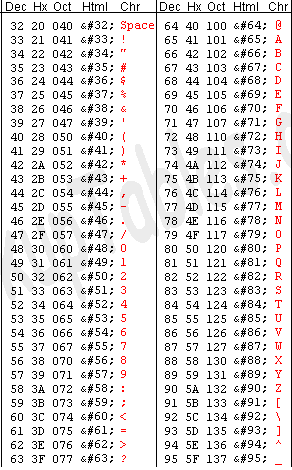
\includegraphics[height=0.7\textheight]{ASCIITABLE}
	\caption{Taken from: http://www.asciitable.com/}
	\label{fig:ASCII}
	\end{figure}
	

\section{Appendix B: Addition and Multiplication Tables for $\mathbb{F}_{64}$}
	\begin{figure}
	\centering
	
\includegraphics[height=\textheight,center]{AddTable}
	\caption{The addition table for $\mathbb{F}_{64}$}
	\label{fig:AddTable}
	\end{figure}
	
	\begin{figure}
	\centering
	
\includegraphics[height=\textheight,center]{MultTable}
	\caption{The multiplication table for $\mathbb{F}_{64}$}
	\label{fig:MultTable}
	\end{figure}
	
	\begin{figure}
	\centering
	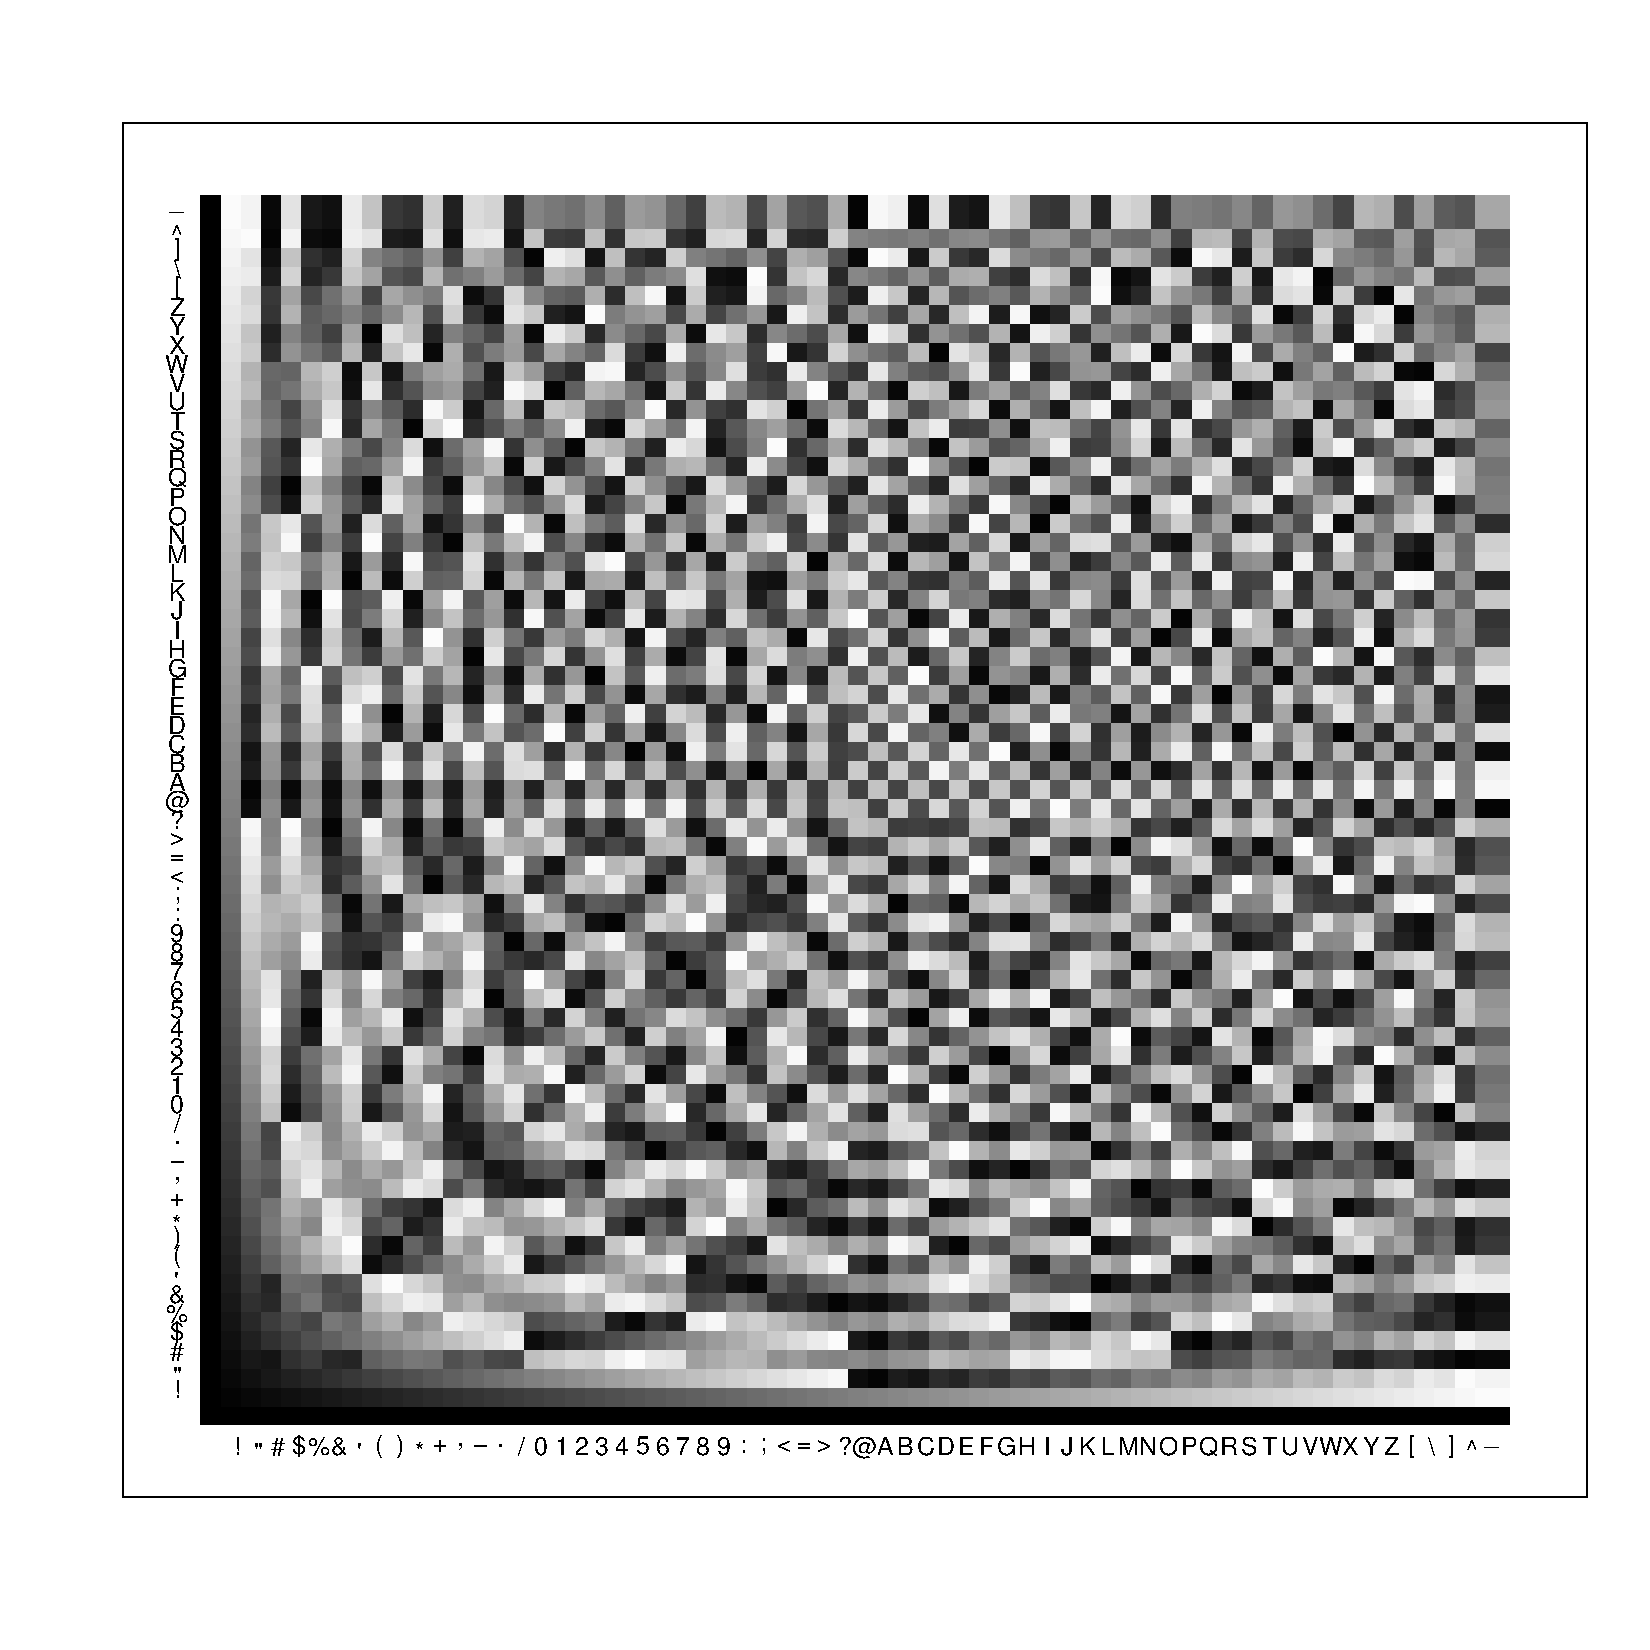
\includegraphics[height=\textheight,center]{GreyScaleTable}
	\caption{A grey-scale multiplication table for $\mathbb{F}_{64}$}
	\label{fig:GreyTable}
	\end{figure}

\end{document}
